
\doublespacing

%-------------------------------------------
%	Chapter 3: Track Reconstruction
%-------------------------------------------
\chapter{Track Reconstruction}

%H important to help show the bigger picture of my research and the motivation behind the work presented

%Successful particles physics measurements are dependent on an efficient and performant re- construction of the physics objects from the detector measurements. As a community we are always striving to run at the edge of the available detector and computation capabilities to ex- tract the maximum amount of information from the experiments. Tracking detectors are at the core of most collider experiments and track reconstruction is one of the crucial tasks in every reconstruction chain.

%Track reconstruction at its heart is a combinatorial problem, i.e. to find the measurements that originate from the same initial particle from a set of possible combinations. The created particles have a wide range of possible properties, especially different creation vertices and momenta, and their particle trajectories have non-deterministic contributions from material interactions. In combination with inhomogeneous magnetic fields and detector inefficiencies, this leads to the possibility of confusion, fake tracks, etc. . All of these effects depend strongly on the density of the measurements and thus on the collision pile-up. Consequently, with the upcoming upgrade to the High-Luminosity Large Hadron Collider (HL-LHC) the track reconstruction complexity will increase significantly.

In particle physics collider experiments, reconstructing particle trajectories (tracks) in a detector is computationally and intellectually one of the most challenging parts of experimental data analysis. The track finding (aka pattern recognition) problem is to associate individual measurements, known as \textit{hits}, into sequences representing tracks. The created particles have a wide range of possible properties, especially different creation vertices and momenta, and their trajectories have non-deterministic contributions from material interactions. These factors in combination with non-homogeneous magnetic fields and detector inefficiencies can lead to the possibility of confusion and hence the creation of fake tracks. All of these effects depend strongly on the measurement density and the collision pile-up.

The scale of such a problem is enormous; a typical LHC detector contains many thousands of sensors measuring particle positions along their trajectory with a total number of sensor channels up to hundreds of millions. Given that the number of hits can be up to $4 \times 10^{5}$ per event, this indicates that the number of tracks can be several thousands. In addition to this, for on-line event selection events must be reconstructed at a rate between 100 kHz and 1 MHz or more. Tracks are widely used for a variety of downstream applications and is essential in all physics signatures, so their accurate reconstruction is a critical task.   

Existing solutions adopted in many silicon based detectors usually rely on well-established algorithms based on seeded track following and combinatorial Kalman filters \cite{AGOSTINELLI2003250} that are often implemented specifically for each experiment. This stage of the algorithm combines hits from a subset of sensors into short track segments called seeds. The track following stage traces each seed through the detector volume and picks up hits belonging to a seeded track.

While these type of algorithms have proven to be quite powerful in the past, they do not scale favorably. The seed number scales non-linearly with the number of hits, and the corresponding CPU time increase (typically close to cubical) creates huge and ever-increasing demand for computing power. Naturally, the question arises whether new algorithms and different approaches exist that might be better suited to handle the conditions at the HL-LHC.

As the HL-LHC is expected to reach unprecedented collision intensities, this will greatly increase the complexity of tracking within the event reconstruction. The drawback of these past methods motivates investigating novel approaches for track finding, in particular, those based on the machine learning (ML) techniques. The benefits of such an approach could lead to tens of millions of pounds savings in CPU needs over the next 20 years of life of the LHC, as well as benefiting all future collider experiments.

In this chapter, track finding in silicon-based detectors is presented. Section \ref{track-finding-silicon-trackers} outlines a typical workflow for track reconstruction in a multi-element silicon tracker and the parameterisation used for specifying the trajectory of charged particle tracks. Section \ref{trackml-detector} presents the TrackML detector and ML challenge; a realistic detector model used to simulate measured particle hits similar to what is expected of the HL-LHC experiment, as well as new approaches to track reconstruction that arose from the challenge. Finally, graph network architectures and track reconstruction using graph networks is presented in Section \ref{graph-networks}, as a potential solution and optimisation to the track finding problem.

%The aim of this project is to explore track finding methods utilizing a graph-based track model and graph neural networks (GNN). An ML-based algorithm will be used to predict a graph adjacency matrix given the input hit features such as a shape of a charge cluster representing a track position measurement in a silicon detector. The excitation/inhibition rules of individual GNN neurons will be designed to facilitate the “simple-to-complex” approach for “hits-to-tracks” association such that the network starts with relatively “easy” areas of an event with low hit density and gradually progresses towards more complex “hot” areas. To efficiently exploit a priori knowledge about charged particle dynamics the GNN-based algorithm will be using simplified Kalman filters as mechanisms for information propagation and track extraction. 

% first talk about graph building using the ML hit pair predictor and then talk about graph pruning/track extraction using the GNN based algorithm



%--------------------------------------------------
%	Chapter 3: Track finding in Silicon Trackers
%---------------------------------------------------
\section{Track finding in Silicon Trackers}
\label{track-finding-silicon-trackers}

%The reconstructed trajectories of charged particles are referred to as tracks. 
%Tracks are reconstructed from the energy depositions (called hits) left by the particles as they traverse the the inner detector.


A typical workflow for track finding in a multi-element silicon tracker such as ATLAS and CMS comprises of a three-stage approach; seeding, track following, and track selection implemented in many current charged particle tracking algorithms. A comprehensive introduction to ATLAS tracking is available in Ref \cite{Cornelissen:2007vba}. An overview of track reconstruction in a multi-element silicon detector is given below.

%The main sequence is referred to as ’inside-out’ track finding, involving clusterisation [17], a CPU-expensive ’track-finding’, followed by precise estimation of track parameters via ’track-fitting’.


%--------------------------------------------------
%	Chapter 3: Track Reconstruction
%---------------------------------------------------
\subsection{Track Reconstruction}
\label{track-reconstruction}

%Describe a typical workflow for track finding in a typical multi-element silicon tracker such as ATLAS and CMS. This workflow is basically a three-stage approach with the seeding, track following, and track selection implemented in the current charged particle tracking algorithms. This is precisely the right place to introduce the TrackML setup. Add that the high-lumi LHC motivates the R\&D of new track finding techniques and we need an environment for fast prototyping and testing various techniques which would allow expert from outside HEP to contribute hence the TrackML.

%This section should be all about track finding in ATLAS, including the main pipeline outlining space-point formation (clustering), track finding (combinatorics), ambiguity solving, neural network cluster splitting, pattern recognition techniques, Kalman filters etc 


\subsubsection{Space-point Formation (Clustering)}
When a charged particle traverses a silicon layer, charge can be deposited in more than one pixel or strip. This is due to the incident angle of the particles with respect to the sensor and also the drift of electrons between sensors caused by their interaction with the magnetic field. Clusters (also called \textit{hits} or \textit{space-points}) are formed by grouping neighbouring pixels or strips and estimating locations of space-points using the shape and energy distribution of the clusters. The clusters are then converted into 3D space-points by a coordinate transformation.

\subsubsection{Seeded Track Finding}
Space-points are used to build track seeds. Seeds are defined as a group of three spacepoints located in different detector layers which are geometrically compatible with being part of a track segment. A combinatorial Kalman filter (KF) is used to build track candidates by extending track seeds. The filter can create multiple track candidates per seed, with bifurcations along the track occurring when more than one compatible spacepoint exists on a given layer. In this way, the KF creates an excess of track candidates, which are only required to satisfy basic quality requirements. Track candidates are allowed to reuse or share hits freely (a single hit may be used by multiple track candidates). Typically, the presence of shared hits is a predictor of a bad track due to the high granularity of the ATLAS tracking detectors. At this stage, there can also be a large number of incorrect hits assigned to otherwise good tracks, and additionally large numbers of fake tracks. Fake tracks are those where the majority of associated hits do not originate from the trajectory of any one physical particle, thus comprising of one or more fake seeds. The low quality of tracks at this stage necessitates an ambiguity solving step, in which the highest quality tracks are selected.

\subsubsection{Track Ambiguity Resolution}

The procedure so far has created candidates with potential overlap. In the ambiguity solver of the ATLAS detector, track candidates are processed individually in descending order of a track score in an effort to resolve this overlap. The track score quantifies the likelihood of the track corresponding to the trajectory of a real particle. Scoring uses a number of variables, including the number and positions of hits, the transverse momentum of the track and the fit quality described as the quality of the track as the $\chi^{2}$ divided by the number degrees of freedom on the track. A preference for high transverse momentum tracks promotes the successful reconstruction of the more physically interesting energetic particles, and suppresses the large number of wrong hits assigned to low momentum tracks. Ambiguity solving was introduced as part of the ATLAS New Tracking effort \cite{Cornelissen:2007vba} intended to improve track reconstruction performance in dense environments. 

\subsubsection{TRT Extension}

The successful tracks from the ambiguity solving stage are extended into the TRT if there is a valid set of matching drift circles. A subsequent track refit is performed in order to increase the precision in parameters of the reconstructed track.


%--------------------------------------------------
%	Chapter 3: Track Parameterisation
%---------------------------------------------------
\subsection{Track Parameterisation}
\label{track-parameterisation}

There are several parameterisations of tracks, but since the shape of the charged particle trajectories in a uniform magnetic field is helical, in general five parameters are required to approximate the true trajectory. One such parameterisation is known as perigee given by Eq. \ref{perigee}:

\begin{equation}\label{perigee}
\textbf{p} = (d_0, z_0, \phi, \theta, Q/p_T)
\end{equation}

The respective transverse and longitudinal impact pararameters (IP); $d_0$ and $z_0$ specify the distance of closest approach of the trajectory of a particle. $\phi$ is the azimuthal angle - the angle in the $x$-$y$ plane and $cot(\theta)$ is the inverse slope of the track in the $(r,z)$ plane, where $\theta$ is the polar angle. $Q/p_T$ is the inverse transverse momentum multiplied by the charge of the particle. Fig. \ref{fig:track-parameters-perigee} shows each of these parameters diagrammatically.


\begin{figure}[!htbp]
  \centering
  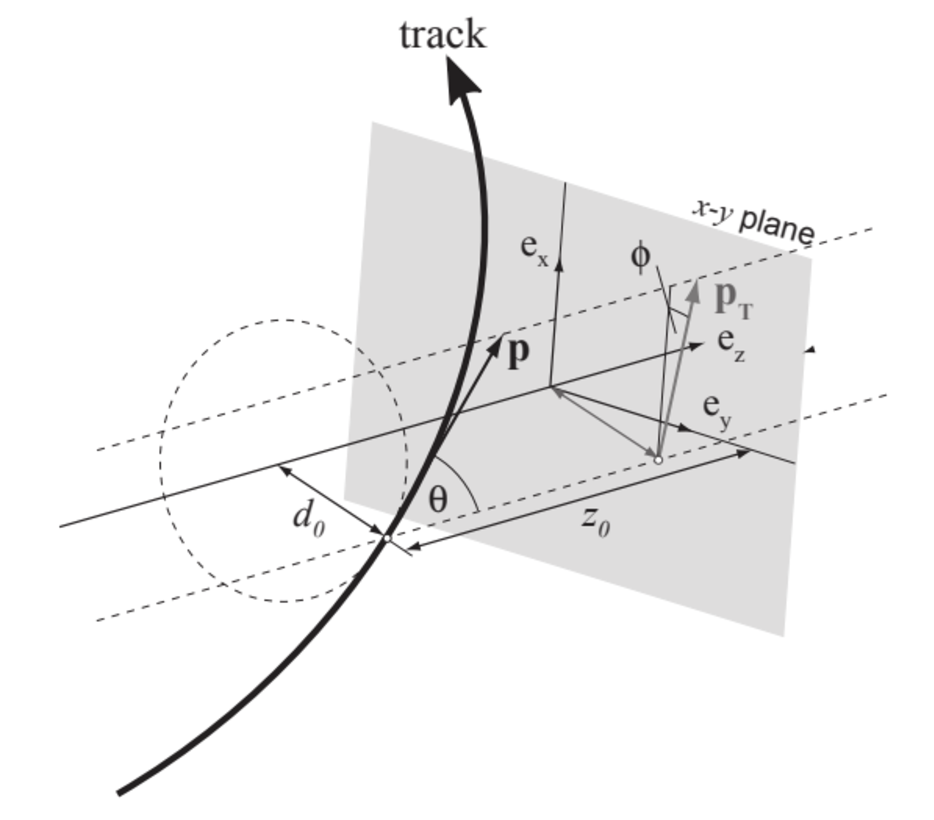
\includegraphics[width=0.65\textwidth]{images/3-track-reconstruction/track_params.pdf}
  \caption{Illustration of the perigee track parameters. Five coordinates are specified $(d_0, z_0, \phi, \theta, Q/p_T)$, defined at the track’s point of closest approach to the nominal interaction point at the origin of the coordinate system. The three-momentum \textbf{p}, transverse momentum $p_T$ (defined in Eq. (\ref{eq:pt})) and basis vectors $e_x$, $e_y$ and $e_z$ are also shown. Reproduced from Ref. \cite{atlastrackingdocs}
  }
  \label{fig:track-parameters-perigee}
\end{figure}


%--------------------------------------------------
%	Chapter 3: TrackML Model
%---------------------------------------------------
\section{The TrackML Model}
\label{trackml-detector}

As the CPU time to reconstruct particle trajectories from measurements is expected to increase faster than the projected computing resources for future detector upgrades, new approaches to pattern recognition are needed to fully exploit the discovery potential of modern silicon detectors. In order to acquire an environment for fast prototyping and developing various techniques, a realistic detector model is needed. As a result, in 2018 a tracking ML challenge was organised on the Kaggle platform; an open-source community platform for data scientists dedicated to the use of challenges as a research tool. The \textit{TrackML Particle Tracking Challenge} \cite{kaggle-trackml} was held in an effort to spark new ideas and algorithmic approaches towards track reconstruction.

The basis of the challenge is using a realistic detector model, develop an algorithm for tracking trajectories of particles using machine learning techniques. The TrackML model simulates measured particle hits similar to what is expected for a HL-LHC experiment and the corresponding data contains 8000 collisions to train on, where each collision has up to 100,000 hits. The participants of the challenge were tasked with connecting these hits into approximately 10,000 arcs of circles, following the trajectory of particles issued from truth data from high energy proton collisions. 

There are many different approaches explored within the TrackML challenge, where the definition of a track determined the most effective approach to use. For example, for a track defined as a point-like object in a parameter space, clustering algorithms would be most appropriate. Whereas, for a track can modelled as a sequence of hits, a track following algorithm using an iterative predict and update mechanism would be most effective.

The structure of the TrackML detector is shown in Section \ref{trackml-structure}, the simulation of the model is discussed in Section \ref{trackml-simulation} and a summary of the challenge algorithms that is beneficial for this thesis is presented in Section \ref{trackml-key-findings}. The TrackML detector is also used for the development of the Graph Neural Network (GNN) based algorithm; see Chapter \ref{chapter-gnn} for further information. More information on the TrackML challenge can be found in \cite{Amrouche_2019}.

\subsection{TrackML Detector Structure}
\label{trackml-structure}
The structure of the detector adopts a generic tracker design that takes key concepts from the existing proposals from ATLAS and CMS detectors. Many modern particle detectors include extensive silicon tracking systems arranged in thin layers of silicon sensors. The TrackML detector is very similar in structure to that of modern detectors and current ATLAS detector known as the ITk \cite{inner-detector-TDR}. It uses a cylinder-like geometry in the central regions and a disk-like geometry in the forward regions. The full detector geometry is shown in Figure \ref{fig:trackml-detector-image}. The detector is split into three separate sub-detectors that differ in spatial resolution and passive material. The innermost sub-detector is a pixel detector with a spatial resolution of 50 $\mu$m $\times$ 50 $\mu$m and further out two different strip detectors with short 80 $\mu$m × 1200 $\mu$m and long strips 0.12 mm $\times$ 10.8 mm are placed. Each detector includes realistic module geometries with placement and overlap chosen to yield a hermetic coverage up to $\lvert \eta \rvert$ = 3.

%ITK: There is no reason to believe the more complex geometry would lead to radically different algorithms

%The TrackML detector also shares several interesting features with the ATLAS detector, for example its solenoid parameters are the same and ....

%Instead of using the proposed upgrade tracker designs of either ATLAS or CMS we opted to design a generic tracker design that takes the key concepts from the existing proposals. This avoids issues of private collaboration information or artefacts and allows a challenge that is more separated from the particular design choices made by each experiment.

% -------------------------------
%More details in the documents on the TrackML competition:
%https://hal.inria.fr/hal-01745714/document
%https://arxiv.org/pdf/1904.06778.pdf
% ------------------------------


\begin{figure}[!htbp]
  \centering
  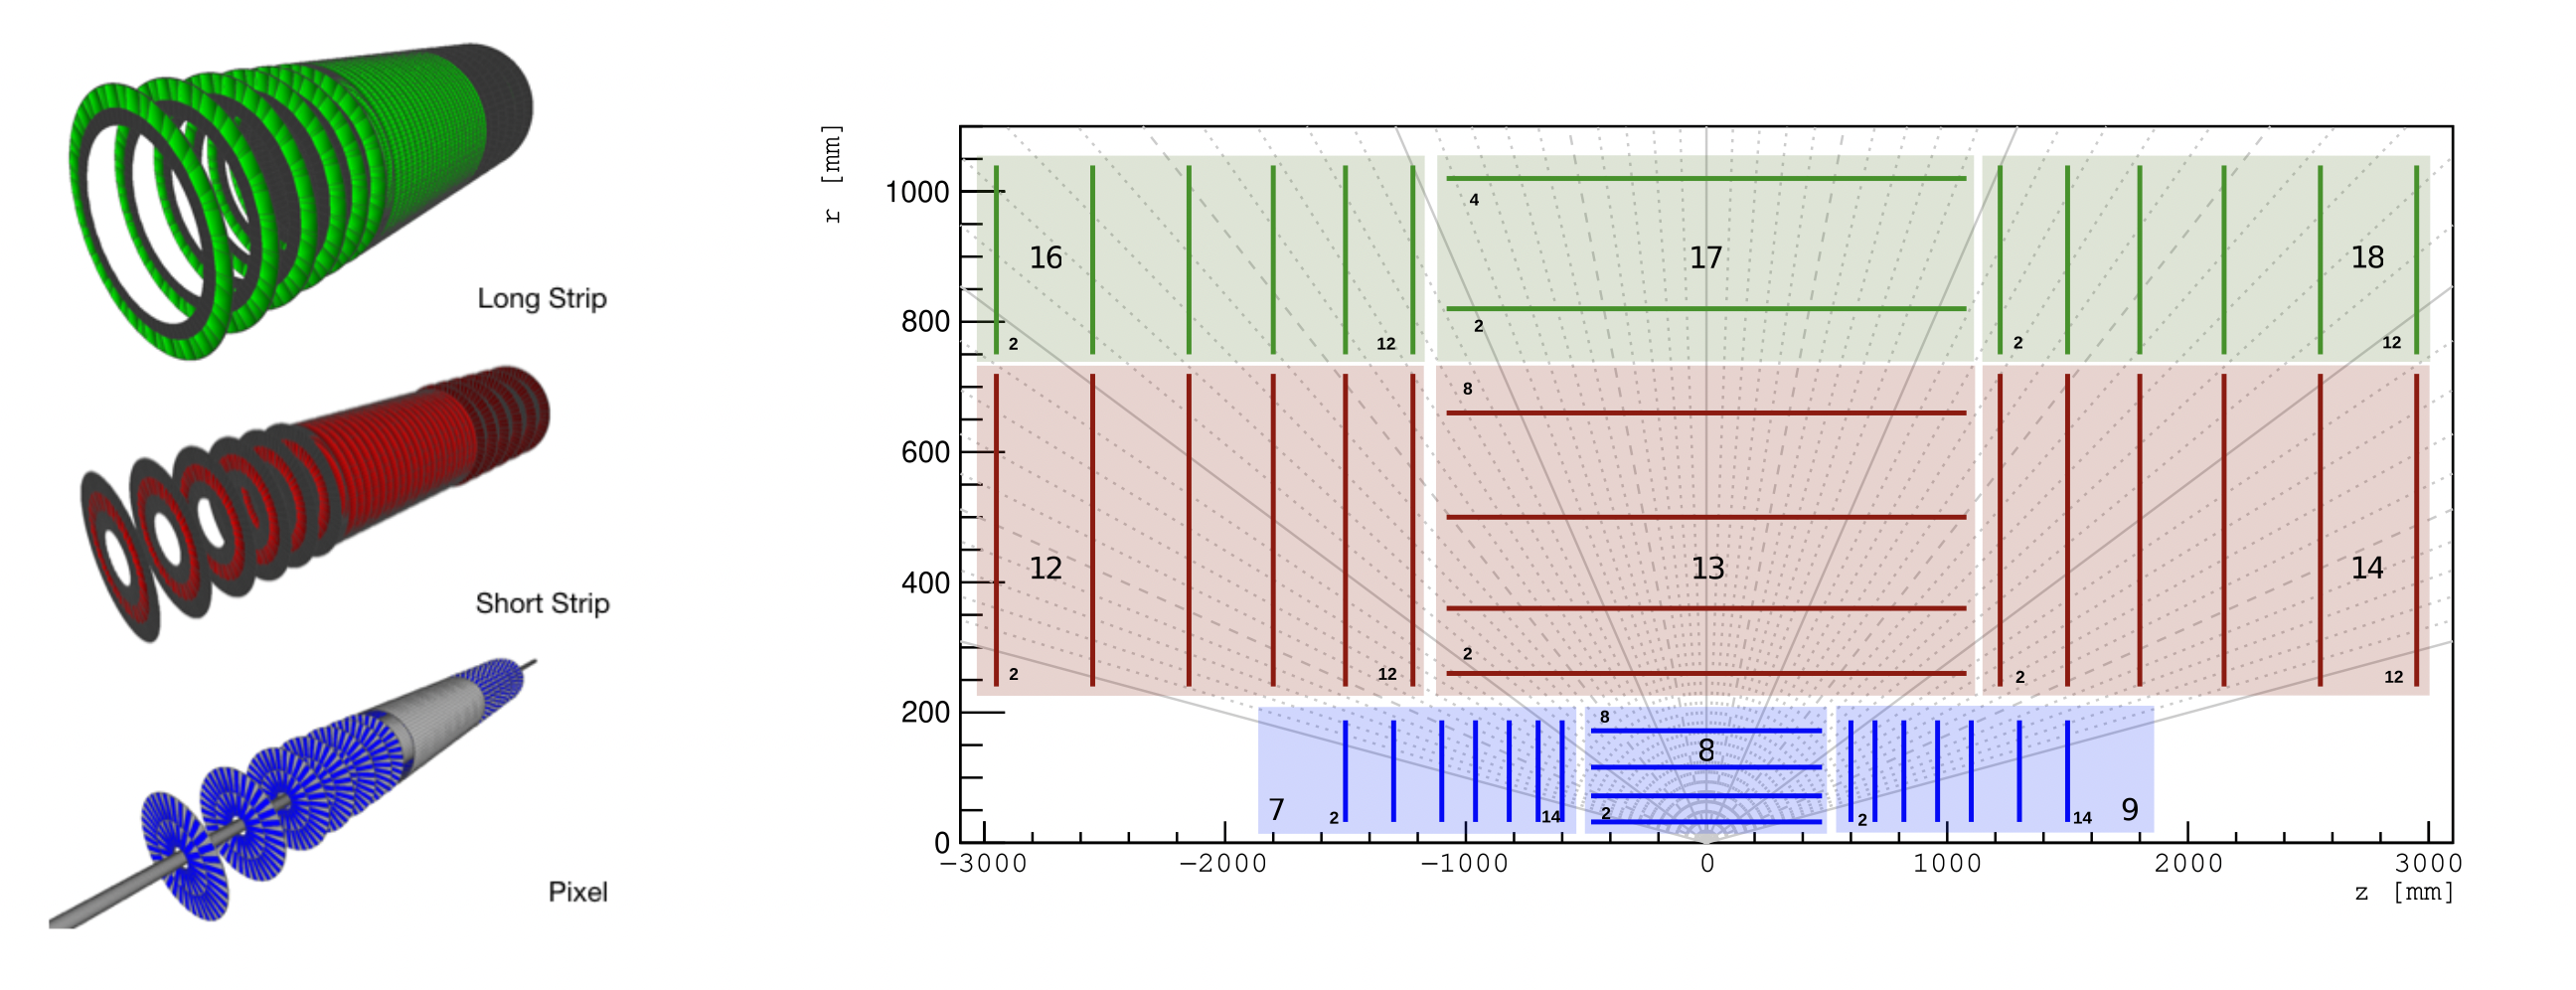
\includegraphics[width=\textwidth]{images/3-track-reconstruction/trackml-detector.png}
  \caption{
    Detector layout for the virtual TrackML detector. On the left the three major sub-detectors, pixel, short strips, and long strips, are shown separately. On the right, a schematic of the full layout and its coverage along the radial and longitudinal dimensions as well as in the $ \lvert \eta \rvert$ direction is shown. The different colors represent the different sub-detectors while the marked numbers are the internal volume and layer identifiers.
  }
  \label{fig:trackml-detector-image}
\end{figure}

\subsection{Event Simulation}
\label{trackml-simulation}
%10.1051_epjconf_201921406037.pdf
The particle content of the collisions is generated using the Pythia 8 event generator \cite{pythia-8}. A hard QCD interaction that generates a $t\bar{t}$-pair is used as the signal. An additional 200 soft QCD interactions are overlayed to simulate the expected pile-up conditions at the HL-LHC. Charged particles are propagated through the detector using a fast detector simulation based on the ACTS software \cite{Gumpert_2017}. A non-homogeneous magnetic field similar to the one in the ATLAS experiment is used and material interactions, i.e. multiple scattering, energy loss, or hadronic interactions, are simulated using parametric models. Only tracks with a transverse momentum above 150 MeV are propagated. Tracks below this momentum threshold are typically not considered by the HL-LHC experiments.

% top quark decays: https://en.wikipedia.org/wiki/Top_quark

\subsection{Challenge Summary and Outlook}
\label{trackml-key-findings}

\subsubsection{Review of Submitted Algorithms}
The competition exposed a diverse range of ML approaches, where accuracy and throughput was used to categorise the best algorithms for track reconstruction. The reconstruction efficiency for a good algorithm is calculated using both track purity and particle purity, and is based on ones that performed best for tracks originating from a low radius near the beam axis and where primary particles are created. The quality of the top performing algorithms were analyzed in further detail. It was found that methods based on track following techniques are highly effective at reconstructing tracks globally with high purity, in comparison with clustering based approaches. 

Amongst the top ranking and winning solutions, the developed algorithms were highly inspired from traditional track following approaches, such as the procedure outlined in Section \ref{track-reconstruction}. The winning algorithm is based on a modular track following strategy, where the definition of a track is given by a sequence of hits. It begins with seed generation selected from hit pairs (doublets) in the innermost layers of the detectors. A logistic regression classifier is trained on doublet features and allows to reduce the number of fakes. These doublets are then extended to triplets via a further logistic classifier trained on triplet features. Track following is then implemented using a helix extrapolation and track ambiguity resolution is executed to remove polluting hits.

% Tracks are then consolidated by taking into account any hits located on overlapping modules if they are closer than a threshold.

Another top performing algorithm is based on training a multi-layered perceptron (MLP) to predict any two hits that are connected to the same track, where the definition of a track is the same as above. All pairs of hits were considered and 27 features were constructed from its quantities. A neural network model composed of multiple wide dense layers is trained to predict the probability of the pair to be on the same track. The proposed approach is an unstructured track following algorithm where the next hit is not provided by track extrapolation, but directly by a hit index based on the hit pair classifier score. This suggests that too many branches of the combinatorial tree are followed during the track following step. Both of the above algorithms yielded high track reconstruction efficiencies of $> 90\%$ (both track purity and particle purity defined as $> 50\%$).

% There is a large class imbalance in the problem due of the predominance of pair of hits that are not belonging to the same track. This is overcome by sampling pairs from the negative class closer to the positive pairs to better define the boundary between the two classes. The accuracy weighted by the class cardinal is a better estimator of the performance of the model in this heavy imbalanced setup.

Another team used various techniques based on the famous clustering-based approach DBSCAN (Density-Based Spatial Clustering of Applications with Noise) \cite{dbscan}. The idea of the DBScan-based algorithm was to find a subspace of track parameters in which a good track could be represented as a point-like object in this subspace. This type of transform is a highly complex task and despite a best effort, the proportion of good tracks reconstructed was $\simeq$ 50\%. 

An alternative methodology implemented by a different team included the use of a recurrent artificial neural network (RNN) using long short-term memory cells (LSTM). This approach begins with seed building, where the DBSCAN algorithm is used to cluster hits in the inner-most layers of the detector in order to produce track seeds. The RNN is used in place of a propagator (such as a traditional KF track following algorithm) to find the potential position of hits on subsequent layers of the detector. The RNN model is trained using multiple architectures and used to predict the positions of the next hits, however the training of the models is quite prohibitive to allow for a full optimization due to its computational load. The proportion of good tracks reconstructed from this algorithm was $\simeq$ 85\%. More information about the details of the competition criteria, analysis and algorithm breakdown can be found in \cite{Amrouche_2019}.

\subsubsection{Motivation for Graph Neural Network Approach}
Several approaches highlighted by the TrackML challenge show great promise for accurate track reconstruction. However in realistic detector setups, the physics reach of particle detectors will be limited by how efficiently the experiments can use their available computing resources. Many of the teams which applied deep learning to the vast amount of training data in the challenge faced computation resource limitations. Even with the use of general purpose Graphical Processing Units (GPUs), training of the models took multiple days. These approaches would not be suitable to implement in the software for realistic detectors.

In addition, approaches that heavily rely on the use of clustering are also not effective for realistic detectors. Clustering based techniques require finding a parameter space where tracks exists as point-like objects. If a detector model contained a perfect uniform magnetic field and there were no material effects present, the behaviour of tracks in such a parameter space could be easily modelled as points and hence algorithms such as DBScan would be highly effective. However, this is not the reality due to multiple scattering effects. Clustering based approaches are widely used to combine hits into doublets and extend doublets to triplets, however they are not the most successful when used to reconstruct tracks globally. The above factors were considered when exploring an alternative route.

In recent years, algorithms for track pattern recognition based on graph neural networks (GNNs) have emerged as a particularly promising route. Early work in this domain focused on establishing a proof of principle, as well as training MLPs and establishing deep learning techniques. 

In the present document a novel methodology is investigated exploring the use of a GNN architecture as a solution to the track pattern recognition problem, without the traditional deep learning approach. The procedure taken is somewhat of an intermediary of the above described algorithms submitted to the TrackML challenge. The GNN-based model presented in this thesis is used to model tracks as sequences of points in a parameter space and simultaneously allows the natural structure of particle trajectories to be embedded into its architecture. The training involved in this procedure is such that functions used to calculate track state parameters are learned, without the need for deep learning or vast computational resources. This approach ensures a realistic implementation for detector experiments. More information on graph network architectures is presented in Section \ref{track-recon-graph-networks}. The development and implementation of the GNN-based algorithm is discussed in Chapter \ref{chapter-5}.

%From the ML point of view, the problem can be treated as a \textbf{latent variable problem} similar to clustering, in which particle trajectory “memberships” must be inferred, a \textbf{tracking problem} considering trajectories as time series, or a \textbf{pattern de-noising problem} considering that the dotted trajectories are noisy versions of continuous traces. As a result the competition exposed a diverse range of ML approaches.

% One important point is that the points on one trajectory are not geometrically close to each other (a human cannot associate the points by eye), but they follow a specific pattern : a distorted arc of helix pointing approximately to the origin.

% Tracking efficiency is commonly defined in particle physics as the probability to reconstruct a track. A good tracking algorithm must provide consistently high efficiency over a wide range of track parameters.


%--------------------------------------------------
%	Chapter 3: Graph Networks
%---------------------------------------------------
\section{Graph Networks}
\label{graph-networks}

Graph network structures are data representations that describe objects and their pairwise relationships. Graphs are able to effectively capture complex relationships and dependencies between such objects, both on a local scale and globally. This is essential for accurately representing physical data and understanding the interactive behaviour of the network. As a result GNNs can represent many types of relational and geometric data. Due to their great expressive power, GNNs have been applied in numerous different applications. They have emerged as the de facto standard for many geometry heavy applications, such as molecular property prediction within drug interactions and social network analysis.

As graph-based architectures are a natural way to represent tracks, they have shown substantial promise for a variety of particle physics tasks. This includes track reconstruction and simulation. In some cases GNNs have demonstrated better scaling properties, reduced resource utilization and increased opportunity for parallel implementation compared to traditional methods.

Section \ref{properties-graph-networks} presents the properties and common terminology used within the domain of graphs networks and \ref{track-recon-graph-networks} introduces the track reconstruction methodology using GNNs investigated in this thesis.

% Useful links!!
% https://www.datacamp.com/tutorial/comprehensive-introduction-graph-neural-networks-gnns-tutorial
% https://distill.pub/2021/gnn-intro/


%--------------------------------------------------
%	Chapter 3: Properties of graph networks
%---------------------------------------------------
\subsection{Properties of Graph Networks}
\label{properties-graph-networks}

\subsubsection{Graph Network Architecture}

A graph is defined by a set of \textit{nodes} \{V\} (or vertices) and a set of \textit{edges} \{E\}. Nodes represent entities or objects and edges are connections between two nodes that model their pairwise relationship. These edges can be directed, non-directed and/or weighted, see Figure \ref{fig:graph-architecture-example} for example illustrations. The connectivity of a graph can be visualized through its adjacency matrix $A \in \{0, 1\}$, of size $n_{nodes} \times n_{nodes}$. If two nodes share an edge, then these entries are populated with 1. 

The data from a tracking detector for a given event can naturally be represented using a graph. A node can represent a hit (or a group of close proximity hits) with each node containing attributes such as spatial coordinates, and the existence of an edge between two nodes indicates that the nodes could potentially represent two successive hits on a track. At the HL-LHC, $O(10^{5})$ hits per $t\bar{t}$ event are expected. A fully connected graph of such an event would have $O(10^{10})$ edges, most of them representing unphysical connections. Therefore, a key feature within graph construction is the choice of compatible edges. 

\begin{figure}[!htbp]
  \centering
  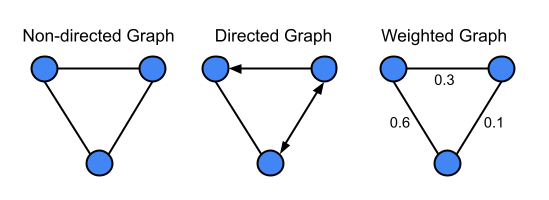
\includegraphics[width=0.85\textwidth]{images/3-track-reconstruction/Graphs.png}
  \caption{
    Illustration of different graph types. Non-directed graphs contain edges with no direction. Directed graphs can contain edges with unidirectional or bidirectional edges. Weighted graphs associate a weight to each edge, the example above has normalised edge weights. All three graphs are fully connected, whereby a unique edge connects each pair of nodes.
  }
  \label{fig:graph-architecture-example}
\end{figure}


\subsubsection{Message Passing Paradigm}

Message passing is an important property in the design of graph networks. It allows the propagation of node features by exchanging information between adjacent nodes. The edges between nodes act as conduits, allowing the transfer of information in a given direction if the connection is active. Typically, this scheme is iterative in nature. It begins with an initialization of states at each node. The node $v$ then aggregates messages from its local neighbourhood. Node representations are then updated based on an aggregation function, improving the precision of states local to each node. This process is then repeated with further message passing and neighbourhood information aggregation, allowing local information to spread globally throughout the network. GNNs can fully exploit the connectivity of its structure, and as a result the mechanism allows models to become sophisticated in learning both local and global behaviour. With the correct application, this type of framework has proved to be highly effective in ML. More information about message passing networks can be found in ..


%--------------------------------------------------
%	Chapter 3: Track reconstruction on graph networks
%---------------------------------------------------
\subsection{Track Reconstruction on Graph Networks}
\label{track-recon-graph-networks}

In this thesis a novel methodology is investigated exploring the use of a GNN architecture as a solution to the track pattern recognition problem. There are two main aspects to this approach; a procedure to construct a graph network is presented in Chapter \ref{chapter-4} and a method to refine its connections and extract tracks is presented in Chapter \ref{chapter-5}. 

In order to identify compatible connections, a ML-based algorithm is used to predict the graph adjacency matrix, given the input hit features such as shape of a charge cluster. An iterative procedure allows ambiguities in the network to be identified and tracks to be isolated. To efficiently exploit a priori knowledge about charged particle dynamics the GNN-based algorithm uses simplified KFs as mechanisms for information propagation as well as for track extraction. 

% In order to build the graph network, a ML-based algorithm will be used to predict the graph adjacency matrix, given the input hit features such as shape of a charge cluster representing a track position measurement in a silicon detector.

%Traditional MLP Training - ExaTrkX and others
% considering previous approaches and new ideas that stemmed from TrackML --> this led to my research
% Then move onto my research and approach

%Novel Deep Learning Methods for track reconstruction
%- Use GNNs for hit classification and segment classification
%- MLP implementation, deep network, many hidden layers
%- Purity 99.5%, Efficiency 98.7%
%- arXiv: 1810.0611, Hep.TrkX Project

%Accelerated Charged Particle Tracking with Graph Neural Networks on FPGAs
%- arXiv:2012.01563
%Graph Neural Networks for Particle Tracking (https://exatrkx.github.io)
% https://arxiv.org/pdf/2203.12852.pdf  - reconstruction section